\speciestitle{Peroxy Radical}{\ch{HO2}}{HO2}{%
  \item[Useful range:] 22--0.046\,hPa
  \item[Product lead:] Luis Mill\'an \email{Luis.F.Millan@jpl.nasa.gov}}

\subsection{Introduction}
MLS observes \ch{HO2} emission lines within the 640-GHz radiometer. A description of \ch{HO2} data quality, precision, systematic errors, and validation for an earlier version, \vii, is given by \citet{PickettEtal:2006:Validation}. An early validation using v1.5 software is also described by \citet{PickettEtal:2006:Validation}. The estimated uncertainties, precisions, and resolution for \thisv \ch{HO2} are summarized below in Table~\ref{tab:HO2Summary}.  

An algorithm to retrieve daily zonal means of \ch{HO2} over an extended vertical range by first averaging the radiances has been developed by the MLS team \citep{MillanEtal:2015}. This alternative dataset provides daytime and nighttime \ch{HO2} measurements across the stratosphere and mesosphere. This dataset and associated documentation is available from the GES-DISC with the product short name ``\texttt{ML3DZMHO2}''.

\subsection{Resolution}

Figure~\ref{fig:AvkHO2} shows the \ch{HO2} averaging kernel for daytime at 70\degsym N and the Equator. The latitudinal variation in the averaging kernel is very small. The vertical resolution for pressures greater than 0.1\,hPa is generally about 5\,km.

\subsection{Precision}

A typical \ch{HO2} profile and the associated precisions (for both \prevv and \thisv) are shown in Figure~\ref{fig:HO2profiles}. The profile is shown in both volume mixing ratio (vmr) and density units. All MLS data are reported in vmr for consistency with the other retrieved molecules. However, use of density units (10\cp{6}\,cm\cp{$-$3}) reduces the apparent steep gradient of the \ch{HO2} vertical profile, allowing one to see the profile with more detail. The nighttime \ch{HO2} profile is expected to exhibit a narrow layer near the altitudes of the nighttime OH layer at \mytexttilde82\,km \citep{PickettEtal:2006:NightOH}, which is not shown in Figure~\ref{fig:HO2profiles} since MLS \ch{HO2} data are not recommended for altitudes above 0.046\,hPa (\mytexttilde70\,km). Precisions are such that an \ch{HO2} zonal average within a 10\degsym\ latitude bin can be determined with better than 10\% relative precision with 20 days of data (\mytexttilde2000 samples) for most pressure levels over 22--0.046\,hPa.

\oneverticalavk{HO2}{\ch{HO2}}%

\begin{figure}
  \begin{center}
    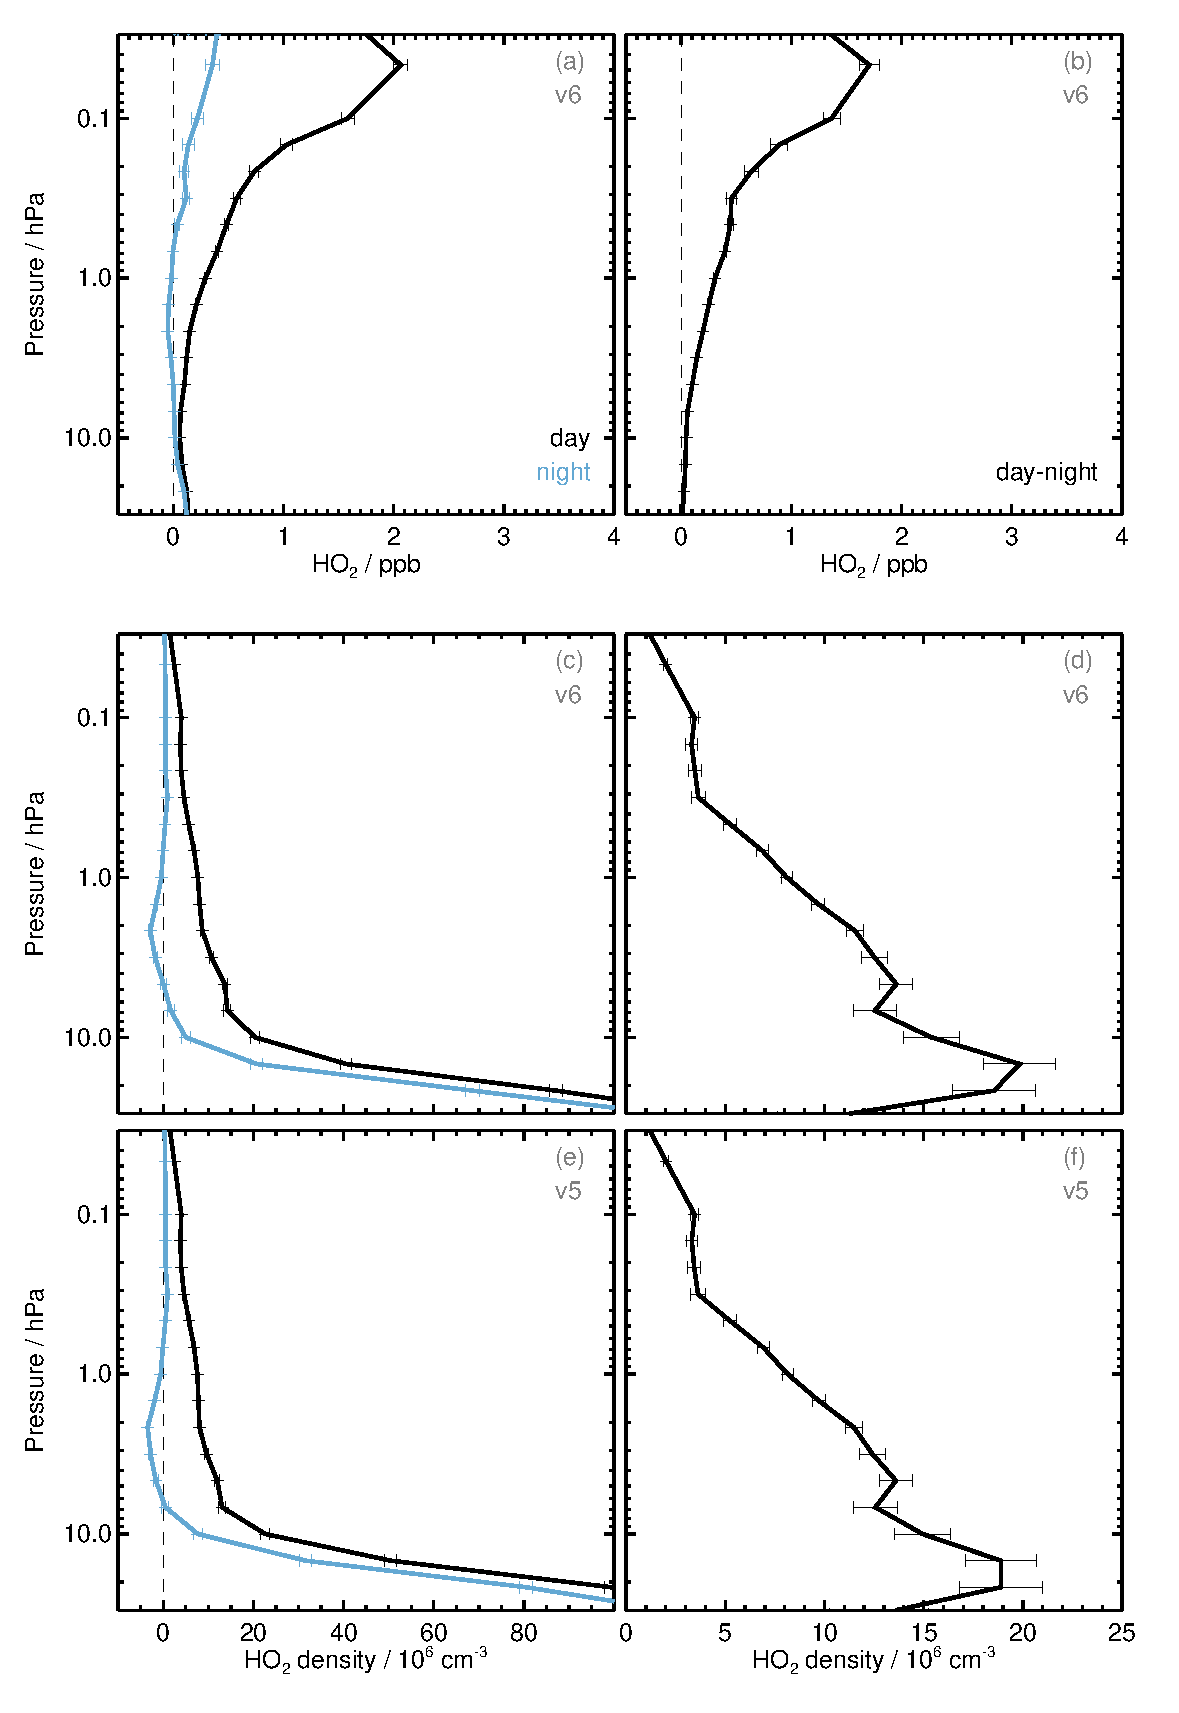
\includegraphics[width=0.8\linewidth]{figures/plot_ho2zmv6.pdf}%
  \end{center}
  \caption{Monthly zonal mean of retrieved \ch{HO2} and its estimated precision (horizontal error bars) for January 2005 averaged over 29\degsym N to 39\degsym N. Panel (a) shows \thisv \ch{HO2} vmr vs.\ pressure for day (black) and night (blue). Panel (b) shows the same data plotted as a day/night difference (note that a day/night difference is required for \ch{HO2} for all pressure levels). Panel (c) shows the same data in (a) converted into density units. Panel (d) shows the day-night differences for the data in panel (c). Panels (e) and (f) are equivalent to (c) and (d) but using \prevv data.}
  \label{fig:HO2profiles}
\end{figure}

\subsection{Accuracy}

Table~\ref{tab:HO2Summary} summarizes the accuracy expected for \thisv \ch{HO2}. The effect of each identified source of systematic error on MLS measurements of radiance has been quantified and modeled \citep{ReadEtal:2007}. These quantified effects correspond to either 2$\sigma$ estimates of uncertainties in each MLS product or an estimate of the maximum reasonable uncertainty based on instrument knowledge and/or design requirements. The \ch{HO2} bias can be minimized by taking day/night differences over the entire recommended pressure range. The overall uncertainty is the square root of the sum of squares of the precision and accuracy.

\begin{nofloatpages}
\subsection{Data screening}
\label{sec:HO2Screening}

\begin{description}
  \item[Pressure range:] \screeningrule{22--0.046\,hPa} \standardrangestatement \standardprecisionrule \evenstatusrule
  \item[Quality:] \screeningrule{MLS \thisv \ch{HO2} data can be used irrespective of the value of the \texttt{Quality} field.}
  \item[Convergence:] \convergencerule{1.1} 
\end{description}
\end{nofloatpages}

\subsection{Artifacts}
Currently, there are no known artifacts in the \ch{HO2} product. The primary limitations are its precision and its narrow recommended altitude range. That said, the alternative daily zonal mean dataset (short name: ``\texttt{ML3DZMHO2}'') offers three distinct improvements over the standard MLS \ch{HO2} product: (1) an extended pressure range, enabling measurements of the mesospheric maximum that occurs near 0.02\,hPa, (2) expanded latitudinal coverage, allowing measurement at the poles, where the \ch{HO2} is located, and (3) nighttime \ch{HO2} estimates.

\subsection{Review of comparisons with other datasets}
\ch{HO2} data from MLS \vii software have been validated with two balloon-borne remote-sensing instruments. Details of the comparison are given by \citet{PickettEtal:2006:Validation}. Comparisons between \vii and \thisv show no differences large enough to alter results of previous validation studies.

\begin{table}
  \caption{Summary of Aura MLS \thisv \ch{HO2} Characteristics}
  \vspace{\tablecaptionsep}
  \label{tab:HO2Summary}
  \begin{minipage}{\linewidth}
    \small\centering\begin{tabular}{ccccl}
\toprule
\tableheaderbox{Pressure\\ \\hPa} &
\tableheaderbox{Vertical\\resolution\\km} &
\tableheaderbox{Single-Profile\\Precision\footnote{Precision (1$\sigma$) on individual profiles as reported in the L2GP files.}\\ \\10\cp6 cm\cp{$-$3}} &
\tableheaderbox{Day--night\\accuracy\\10\cp6 cm\cp{$-$3}} &
\textbf{Comments} \\
\midrule
 $<$ 0.03  & ---   & ---               & ---  &  Unsuitable for scientific use\\
 0.046     & 10    & 4                 & 0.01 &  Use day--night difference \\
 0.10      & 7     & 8                 & 0.3  &  Use day--night difference \\
 1.0       & 5     & 11                & 0.5  &  Use day--night difference \\
 10        & 4     & 56                & 15   &  Use day--night difference \\
 $>$ 22    & ---   & ---               & ---  &  Unsuitable for scientific use\\
\bottomrule
\end{tabular}
  \end{minipage}
\end{table}
